\task{
	Полный заряд параллелепипеда равномерно заряженного по всему объему равен $Q_1$. В результате
    нанесения дополнительного поверхностного заряда $Q_2$ на все грани этого параллелепипеда, кроме грани
    $ABCD$, поле в точке $F$ оказывается равным нулю. Определите величину отношения $Q_2 / Q_1$. Длины
    ребер параллелепипеда указаны на рисунке.
}

\begin{center}
	\tikzstyle{start} = [circle, inner sep = 1pt, opacity = 1]
    \tikzstyle{end} = [circle, fill, minimum size = 0mm, inner sep = 0pt]
    \tikzstyle{path} = [draw, opacity = 1]

    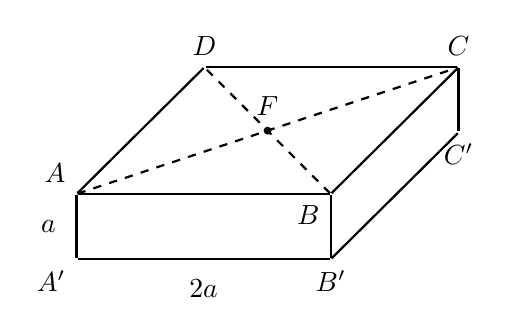
\begin{tikzpicture}[grow = right, thick]
        \def\a{0.8cm}
        \def\k{4}

        \node[end, label = above left:$A$] (A) {};
        \node at (A.south) [end, below = \a, label = below left:$A'$] (A1) {};
        \path[path] (A) -- (A1) node [midway, label = left:$a$] {};

        \node at (A.east) [end, right = \k * \a, label = below left:$B$] (B) {};
        \node at (B.south) [end, below = \a, label = below:$B'$] (B1) {};
        \path[path] (B) -- (B1);

        \path[path] (A) -- (B);
        \path[path] (A1) -- (B1) node [midway, label = below:$2a$] {};

        \node at (A.east) [end, above right = \k * \a / 2, label = above:$D$] (D) {};
        \path[path] (A) -- (D);

        \node at (D.east) [end, right = \k * \a, label = above:$C$] (C) {};
        \node at (C.south) [end, below = \a, label = below:$C'$] (C1) {};

        \path[path] (C) -- (D);
        \path[path] (C) -- (C1);
        \path[path] (B1) -- (C1);
        \path[path] (B) -- (C);
        \path[path, dashed] (B) -- (D);
        \path[path, dashed] (A) -- (C) node [circle, fill, midway, minimum size = 1mm, inner sep = 0pt,
    	    label = above:$F$] {};
    \end{tikzpicture}
\end{center}
